\section{Bevölkerungsdichten der Landkreise und Regierungsbezirke}
In \autoref{fig:distribution_pop_density_counties} sind die Bevölkerungsdichten der einzelnen Landkreise dargestellt. Eine komplette Auflistung der Landkreise in dieser Reihenfolge findet sich \autoref{tab:counties_by_pop_density}.

\begin{figure}[H]
    \centering
    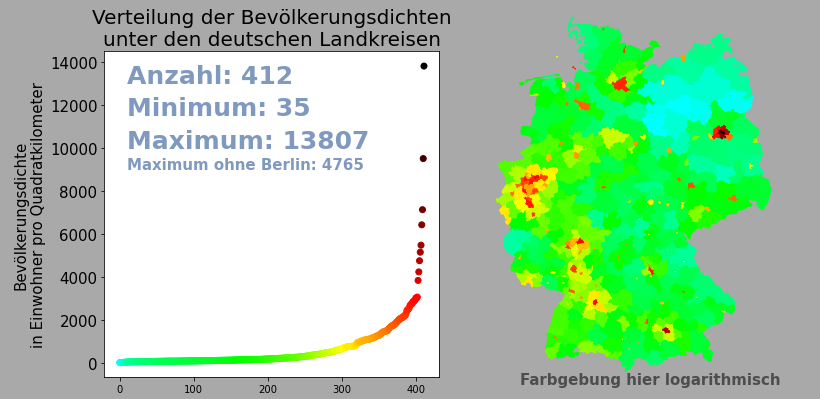
\includegraphics[width = 0.95\textwidth]{figures/Ergebnisse/population_density_counties.png}
    \caption{Verteilung der Bevölkerungsdichten  der deutschen Landkreisen $\rho_{Gebiet}$, wie in Gleichung \autoref{eq:Bevölkerungsdichte} beschrieben. Auf der linken Seite befindet sich die Verteilung, welche zudem die Farbgebung vorgibt. Auf der rechten Seite die räumliche Anordnung. Die Farbgebung entspricht \autoref{sec:Grundlagen:Farbgebung}. Da jedoch wenige Wert sehr hoch sind, wie im linken Teil klar zu sehen, wird der Logarithmus der Bevölkerungsdichte benutzt, um die Farben zu vergeben.}
    \label{fig:distribution_pop_density_counties}
\end{figure}

In \autoref{fig:distribution_pop_density_districts} sind die Bevölkerungsdichten der einzelnen Regierungsbezirke dargestellt. Auf der linken Seite befindet sich die Verteilung und auf der rechten Seite die räumliche Anordnung.

\begin{figure}[H]
    \centering
    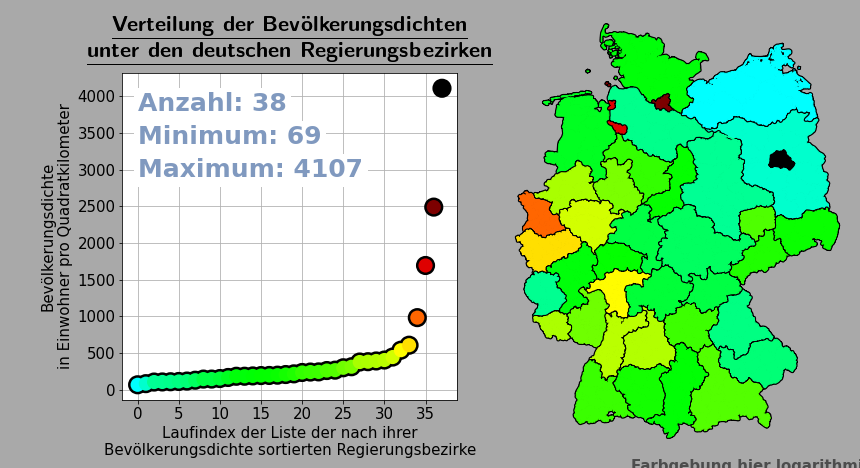
\includegraphics[width = 0.95\textwidth]{figures/Ergebnisse/population_density_ditricts.png}
    \caption{Verteilung der Bevölkerungsdichten unter den deutschen Regierungsbezirken. Die Skalierung entspricht der Farbgebung in \autoref{fig:distribution_pop_density_counties}.}
    \label{fig:distribution_pop_density_districts}
\end{figure}